% TODO: Rename as Result?
\textit{Summarizing the chapter}

% \begin{sidewaystable}
%     \centering
%     \label{tab:common:table}
%     \caption{Common table}
%     \resizebox{\columnwidth}{!}{
%         \input{Data/results/FFT/common_table.tex}
%     }
% \end{sidewaystable}

\begin{table}
    \centering
    \label{tab:common:table:cpp}
    \caption{Common table for C++ tests}
    \resizebox{\columnwidth}{!}{
        \begin{tabular}{|l|c|c|c|c|c|}\hline
\textbf{Block size}  & \textbf{Columbia converted Iterative} & \textbf{Columbia optimized Iterative} & \textbf{KISS} & \textbf{Princeton converted Iterative} & \textbf{Princeton converted Recursive}\\\hline
\textbf{16}  & 0.0225 $\pm$ 0.0033 & 0.0198 $\pm$ 0.0025 & 0.0195 $\pm$ 0.0067 & 0.0342 $\pm$ 0.0053 & 0.0612 $\pm$ 0.0065\\\hline
\textbf{32}  & 0.0322 $\pm$ 0.0025 & 0.0322 $\pm$ 0.0031 & 0.0239 $\pm$ 0.0031 & 0.0545 $\pm$ 0.0043 & 0.1085 $\pm$ 0.0020\\\hline
\textbf{64}  & 0.0525 $\pm$ 0.0014 & 0.0524 $\pm$ 0.0012 & 0.0338 $\pm$ 0.0020 & 0.0847 $\pm$ 0.0059 & 0.2148 $\pm$ 0.0024\\\hline
\textbf{128}  & 0.1025 $\pm$ 0.0033 & 0.0814 $\pm$ 0.0127 & 0.0629 $\pm$ 0.0084 & 0.1328 $\pm$ 0.0029 & 0.4517 $\pm$ 0.0057\\\hline
\textbf{256}  & 0.0925 $\pm$ 0.0178 & 0.0822 $\pm$ 0.0039 & 0.1158 $\pm$ 0.0035 & 0.2807 $\pm$ 0.0073 & 0.9139 $\pm$ 0.0067\\\hline
\textbf{512}  & 0.1709 $\pm$ 0.0267 & 0.1744 $\pm$ 0.0308 & 0.2109 $\pm$ 0.0049 & 0.5486 $\pm$ 0.0253 & 1.9142 $\pm$ 0.0102\\\hline
\textbf{1024}  & 0.3656 $\pm$ 0.0284 & 0.3397 $\pm$ 0.0108 & 0.4072 $\pm$ 0.0086 & 1.1691 $\pm$ 0.0172 & 4.0665 $\pm$ 0.0127\\\hline
\textbf{2048}  & 0.9177 $\pm$ 0.0541 & 0.7402 $\pm$ 0.0190 & 0.8635 $\pm$ 0.0243 & 2.4714 $\pm$ 0.0188 & 8.7235 $\pm$ 0.0725\\\hline
\textbf{4096}  & 1.6737 $\pm$ 0.0461 & 1.9889 $\pm$ 0.0982 & 1.9558 $\pm$ 0.1347 & 5.3867 $\pm$ 0.1000 & 18.3487 $\pm$ 0.1235\\\hline
\textbf{8192}  & 3.7768 $\pm$ 0.1838 & 3.8584 $\pm$ 0.2236 & 3.8499 $\pm$ 0.1603 & 11.7050 $\pm$ 0.5076 & 38.4780 $\pm$ 0.6441\\\hline
\textbf{16384}  & 8.2947 $\pm$ 0.3759 & 8.5556 $\pm$ 0.5672 & 7.8854 $\pm$ 0.2775 & 24.3807 $\pm$ 0.5902 & 80.4920 $\pm$ 0.8228\\\hline
\textbf{32768}  & 19.1886 $\pm$ 1.1809 & 18.5907 $\pm$ 0.9959 & 17.6197 $\pm$ 0.5490 & 52.3713 $\pm$ 1.1313 & 167.3867 $\pm$ 1.5300\\\hline
\textbf{65536} & 42.8520 $\pm$ 1.4120 & 44.2337 $\pm$ 2.4361 & 38.3601 $\pm$ 0.7332 & 112.4273 $\pm$ 1.1197 & 346.7600 $\pm$ 1.9190\\\hline
\end{tabular}

    }
\end{table}

\begin{table}
    \centering
    \label{tab:common:table:java}
    \caption{Common table for Java tests}
    \resizebox{\columnwidth}{!}{
        \begin{tabular}{|l|c|c|c|}\hline
\textbf{Block size}  & \textbf{Columbia Iterative} & \textbf{Princeton Iterative} & \textbf{Princeton Recursive}\\\hline
\textbf{16}  & 0.0210 $\pm$ 0.0008 & 0.1738 $\pm$ 0.0368 & 0.2730 $\pm$ 0.0708\\\hline
\textbf{32}  & 0.0429 $\pm$ 0.0018 & 0.0571 $\pm$ 0.0071 & 0.3983 $\pm$ 0.0568\\\hline
\textbf{64}  & 0.0906 $\pm$ 0.0010 & 0.0916 $\pm$ 0.0073 & 0.2104 $\pm$ 0.0402\\\hline
\textbf{128}  & 0.2233 $\pm$ 0.0382 & 0.2353 $\pm$ 0.0339 & 0.3204 $\pm$ 0.0425\\\hline
\textbf{256}  & 0.0372 $\pm$ 0.0022 & 0.4380 $\pm$ 0.0316 & 0.7415 $\pm$ 0.0431\\\hline
\textbf{512}  & 0.0754 $\pm$ 0.0029 & 0.9865 $\pm$ 0.0672 & 1.7743 $\pm$ 0.1944\\\hline
\textbf{1024}  & 0.1507 $\pm$ 0.0059 & 2.0255 $\pm$ 0.0933 & 3.5339 $\pm$ 0.2466\\\hline
\textbf{2048}  & 0.4299 $\pm$ 0.0312 & 4.5366 $\pm$ 0.3038 & 8.2740 $\pm$ 0.6905\\\hline
\textbf{4096}  & 0.9984 $\pm$ 0.0915 & 10.6191 $\pm$ 0.8679 & 17.9445 $\pm$ 0.9022\\\hline
\textbf{8192}  & 2.3125 $\pm$ 0.2709 & 27.5617 $\pm$ 1.9755 & 37.6118 $\pm$ 1.5008\\\hline
\textbf{16384}  & 4.8597 $\pm$ 0.4114 & 62.6869 $\pm$ 1.7191 & 80.1848 $\pm$ 1.9414\\\hline
\textbf{32768}  & 11.2535 $\pm$ 0.9718 & 155.5247 $\pm$ 2.7411 & 172.5062 $\pm$ 2.2489\\\hline
\textbf{65536} & 26.3906 $\pm$ 2.1662 & 366.0557 $\pm$ 2.8910 & 366.6833 $\pm$ 3.3610\\\hline
\end{tabular}

    }
\end{table}

\begin{table}
    \centering
    \label{tab:java:princeton:iterative}
    \caption{Java Princeton Iterative, Time (ms)}
    /home/algo/Skola/Exjobb/Data/results/FFT/Java_Princeton_Iterative_N_30.tex
\end{table}
\begin{table}
    \centering
    \label{tab:java:princeton:recursive}
    \caption{Java Princeton Recursive, Time (ms)}
    \input{Data/results/FFT/Java_Princeton_Recursive.tex}
\end{table}
\begin{table}
    \centering
    \label{tab:java:columbia:iterative}
    \caption{Java Columbia Iterative, Time (ms)}
    /home/algo/Skola/Exjobb/Data/results/FFT/Java_Columbia_Iterative_N_30.tex
\end{table}
\begin{table}
    \centering
    \label{tab:cpp:princeton:iterative}
    \caption{C++ Princeton Iterative, Time (ms)}
    /home/algo/Skola/Exjobb/Data/results/FFT/CPP_Princeton_converted_Iterative_N_30.tex
\end{table}
\begin{table}
    \centering
    \label{tab:cpp:princeton:recursive}
    \caption{C++ Princeton Recursive, Time (ms)}
    /home/algo/Skola/Exjobb/Data/results/FFT/CPP_Princeton_converted_Recursive_N_30.tex
\end{table}
\begin{table}
    \centering
    \label{tab:cpp:columbia:iterative}
    \caption{C++ Columbia Iterative, Time (ms)}
    \input{Data/results/FFT/CPP_Columbia_converted_Iterative.tex}
\end{table}
\begin{table}
    \centering
    \label{tab:cpp:kiss}
    \caption{C++ KISS, Time (ms)}
    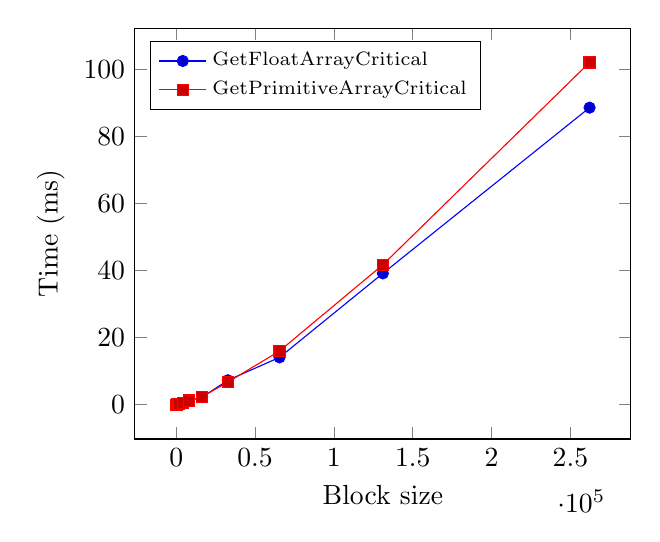
\begin{tikzpicture}
\begin{axis}[xlabel={Block size},ylabel={Time (ms)},width=0.65\linewidth,legend pos=north west,scaled y ticks = false,legend cell align=left,legend style={font=\scriptsize}]
\addplot coordinates {
(16, 0.0050)
(32, 0.0060)
(64, 0.0072)
(128, 0.0139)
(256, 0.0212)
(512, 0.0478)
(1024, 0.0885)
(2048, 0.1965)
(4096, 0.3867)
(8192, 1.1701)
(16384, 2.2685)
(32768, 7.2940)
(65536, 14.1297)
(131072, 39.1887)
(262144, 88.6356)
};
\addplot coordinates {
(16, 0.0056)
(32, 0.0069)
(64, 0.0079)
(128, 0.0131)
(256, 0.0182)
(512, 0.0461)
(1024, 0.0992)
(2048, 0.2047)
(4096, 0.4022)
(8192, 1.2470)
(16384, 2.3713)
(32768, 6.7420)
(65536, 16.0281)
(131072, 41.7620)
(262144, 102.1196)
};
\legend{GetFloatArrayCritical, GetPrimitiveArrayCritical}
\end{axis}
\end{tikzpicture}

\end{table}
\begin{table}
    \centering
    \label{tab:cpp:columbia:iterative:optimized}
    \caption{C++ Columbia Iterative Optimized, Time (ms)}
    \input{Data/results/FFT/CPP_Columbia_optimized_Iterative.tex}
\end{table}

\begin{figure}
    \centering
    /home/algo/Skola/Exjobb/Data/results/FFT/Java_Princeton_Recursive_N_30_barplot.tex
    \label{fig:cpp:columbia:iterative:optimized}
    \caption{C++ Columbia Iterative Optimized bar plot}
\end{figure}
% \begin{table}
%     \centering
%     \label{fig:cpp:columbia:iterative:optimized}
%     \caption{Label here}
%     \input{Data/results/FFT/Java_Columbia_optimized_Iterative.tex}
% \end{table}
